\newpage
\newpage
\anexo{Distribuciones longitudinales de primarios individuales}\label{sec:apendiceC}


Las siguientes gráficas corresponden, cada uno, a distribuciones longitudinales de primarios individuales, usando la atmósfera predeterminada (línea azul), y usando la atmósfera construida para el mes de abril (línea roja). Se observa el número de partículas que se genera, a medida que la EAS se desarrolla a través de la atmósfera (superior izquierda), la diferencia porcentual en relación al número de partículas generadas con la atmósfera predeterminada (inferior izquierda), la energía depositada a lo largo del desarrollo de la EAS (superior derecha), y la diferencia porcentual en relación a la energía depositada con la atmósfera predeterminada (inferior derecha).

\begin{figure}[htb!]
\centering
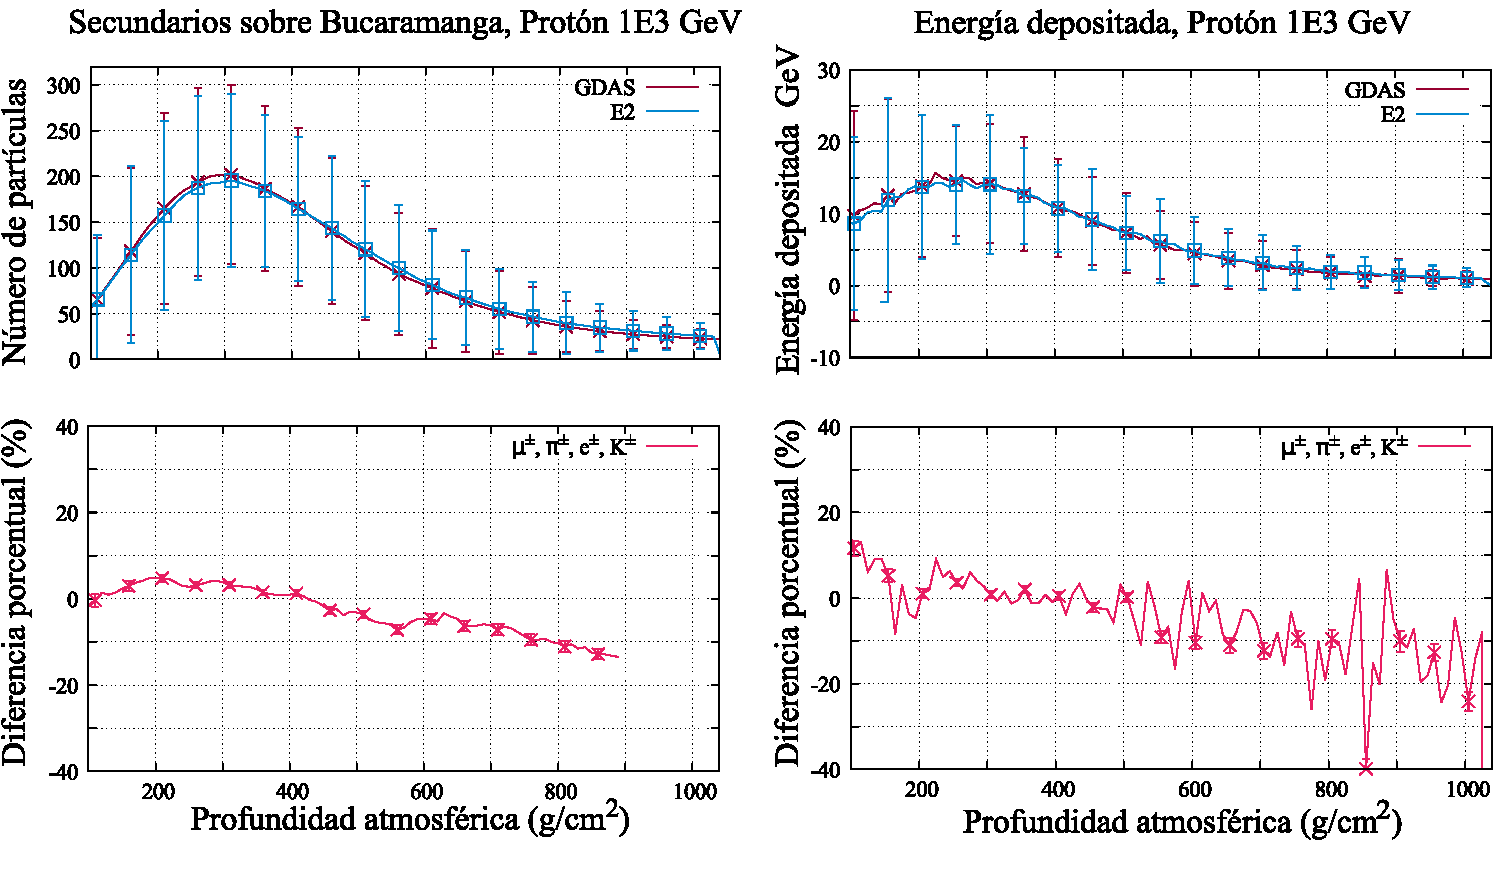
\includegraphics[width=0.8\textwidth]{Figs/proton_1E3.pdf}
\caption[Distribución longitudinal de un protón de $1\cdot 10^{3}$ GeV.]{Distribución longitudinal de un protón de $1\cdot 10^{3} GeV$ que fue simulado 5000 veces, usando la atmósfera predeterminada (línea azul), y usando la atmósfera construida para el mes de abril (línea roja).}
\label{fig:fig26}
\end{figure}

\begin{figure}[htb!]
\centering
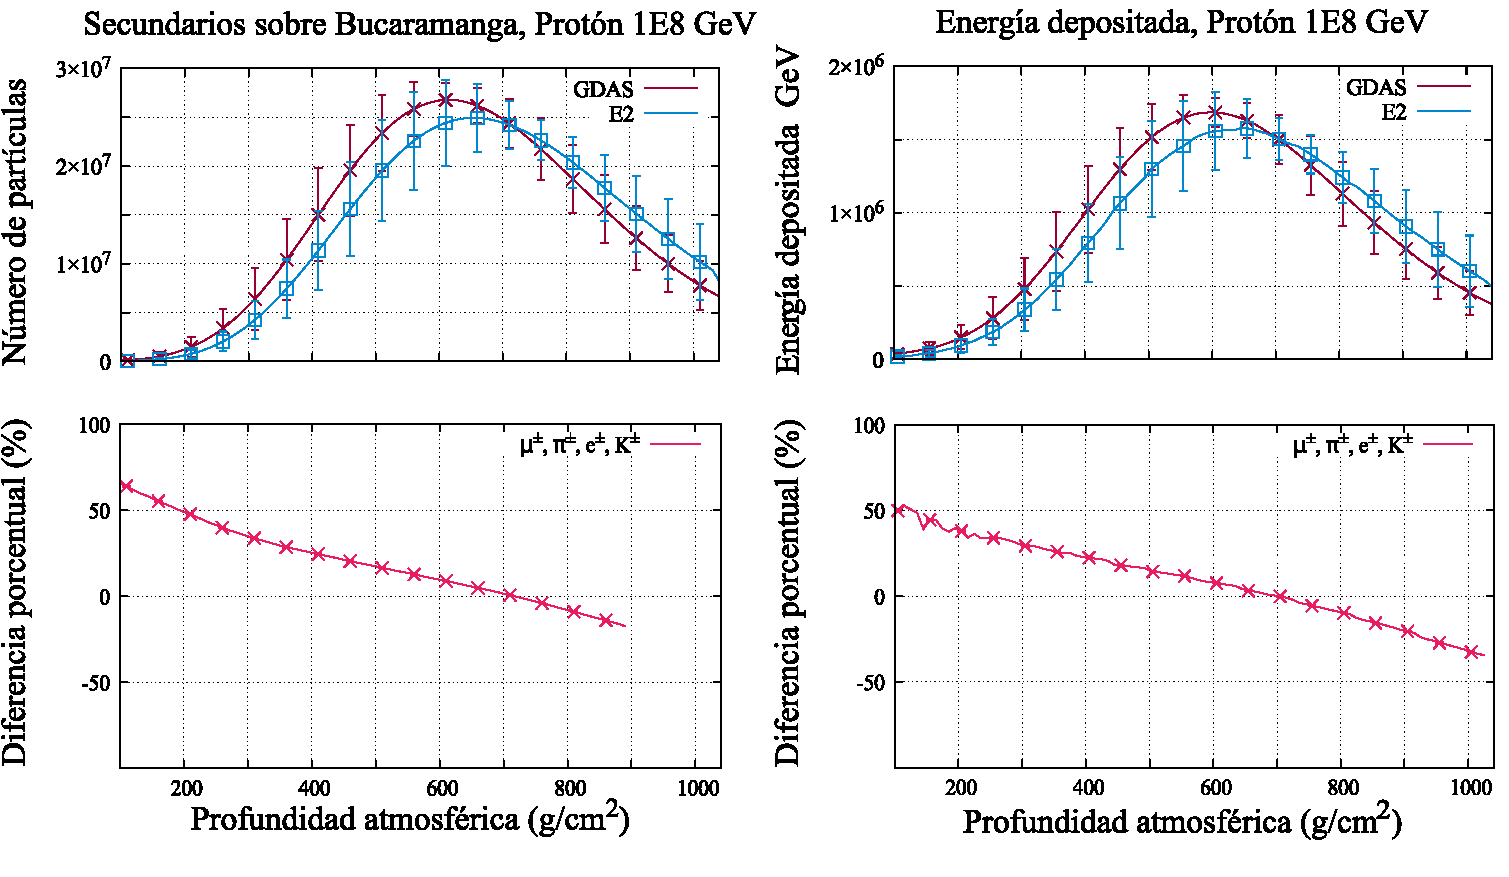
\includegraphics[width=0.8\textwidth]{Figs/proton_1E8.pdf}
\caption[Distribución longitudinal de un protón de $1\cdot 10^{8}$ GeV.]{Distribución longitudinal de un protón de $1\cdot 10^{8} GeV$ que fue simulado 10 veces, usando la atmósfera predeterminada (línea azul), y usando la atmósfera construida para el mes de abril (línea roja). }
\label{fig:fig26b}
\end{figure}


\begin{figure}[htb!]
\centering
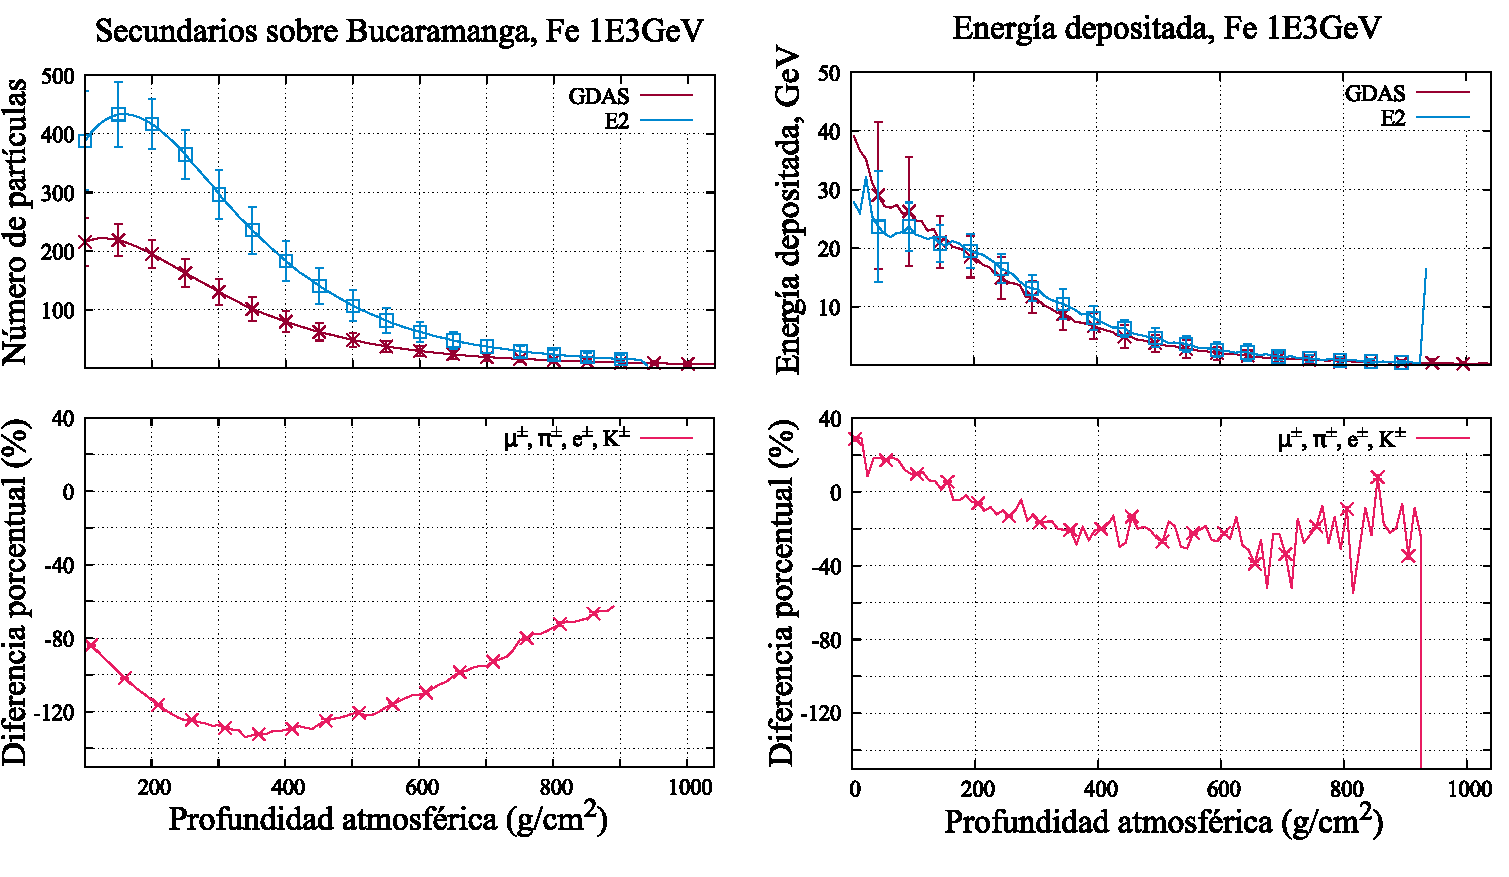
\includegraphics[width=0.8\textwidth]{Figs/fe_1E3.pdf}
\caption[Distribución longitudinal de un núcleo de hierro de $1\cdot 10^{3}$ GeV.]{Distribución longitudinal de un núcleo de hierro de $1\cdot 10^{3} GeV$ que fue simulado 5000 veces, usando la atmósfera predeterminada (línea azul), y usando la atmósfera construida para el mes de abril (línea roja). }
\label{fig:fig27}
\end{figure}

\begin{figure}[htb!]
\centering
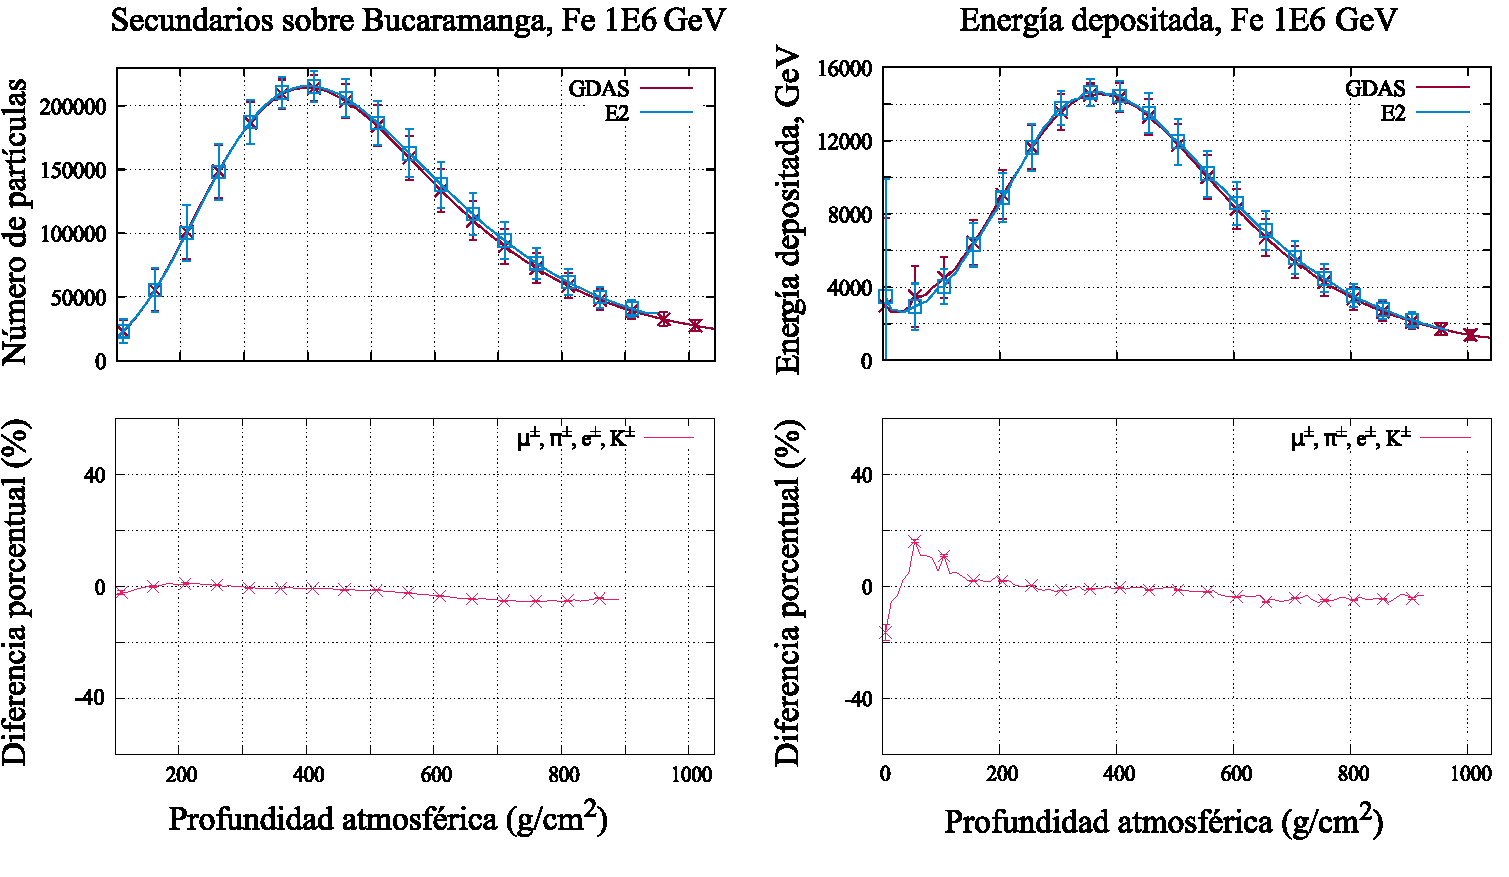
\includegraphics[width=0.8\textwidth]{Figs/fe_1E6.pdf}
\caption[Distribución longitudinal de un núcleo de hierro de $1\cdot 10^{6}$ GeV.]{Distribución longitudinal de un núcleo de hierro de $1\cdot 10^{6} GeV$ que fue simulado 1000 veces, usando la atmósfera predeterminada (línea azul), y usando la atmósfera construida para el mes de abril (línea roja). }
\label{fig:fig28}
\end{figure}

\begin{figure}[htb!]
\centering
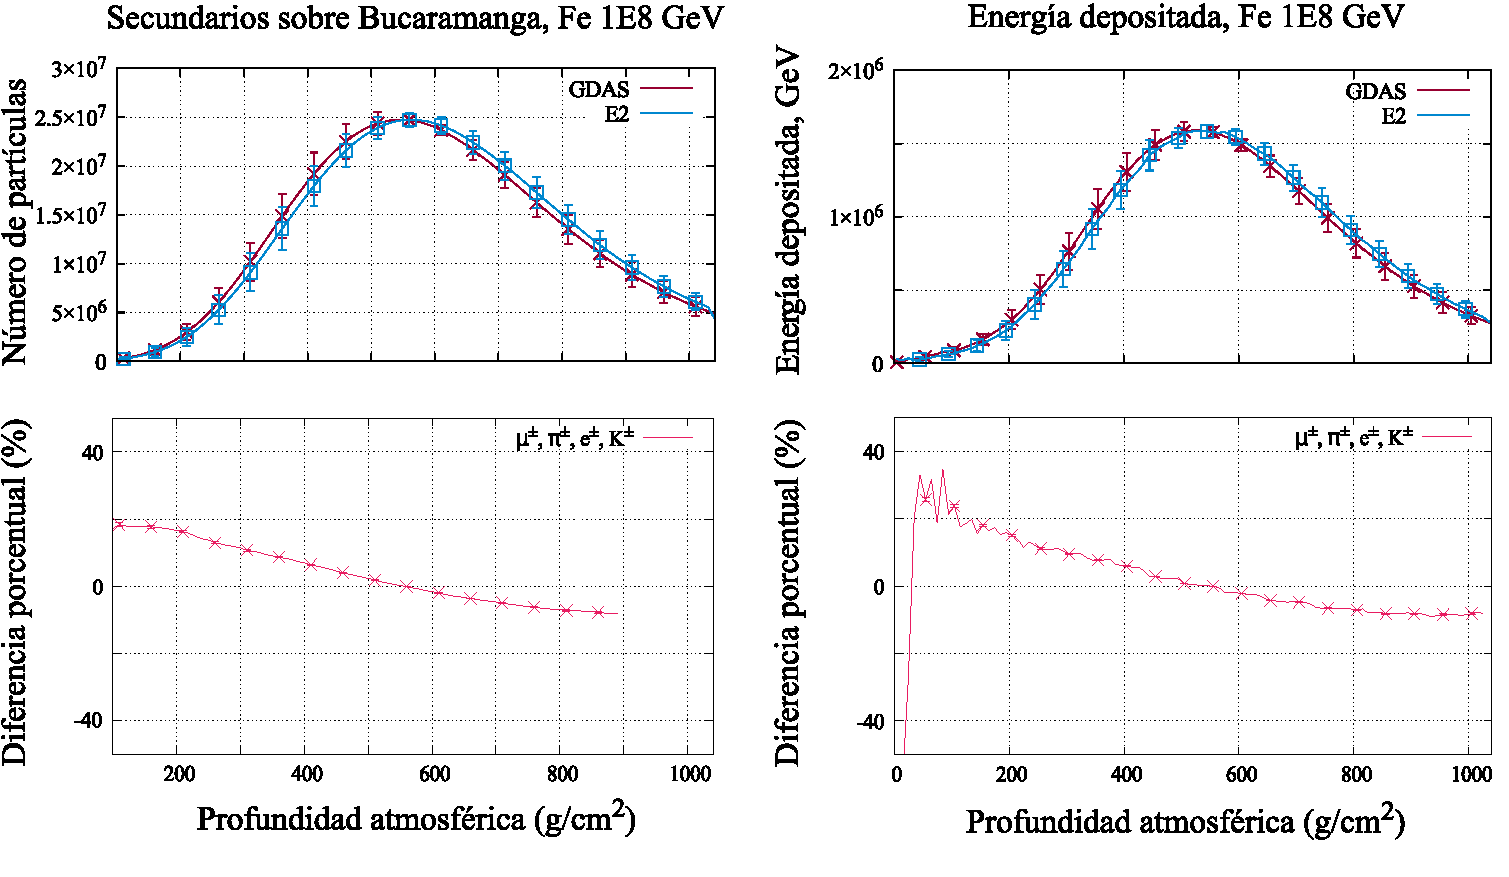
\includegraphics[width=0.8\textwidth]{Figs/fe_1E8.pdf}
\caption[Distribución longitudinal de un núcleo de hierro de $1\cdot 10^{8}$ GeV.]{Distribución longitudinal de un núcleo de hierro de $1\cdot 10^{3} GeV$ que fue simulado 10 veces, usando la atmósfera predeterminada (línea azul), y usando la atmósfera construida para el mes de abril (línea roja). }
\label{fig:fig29}
\end{figure}

\begin{figure}[htb!]
\centering
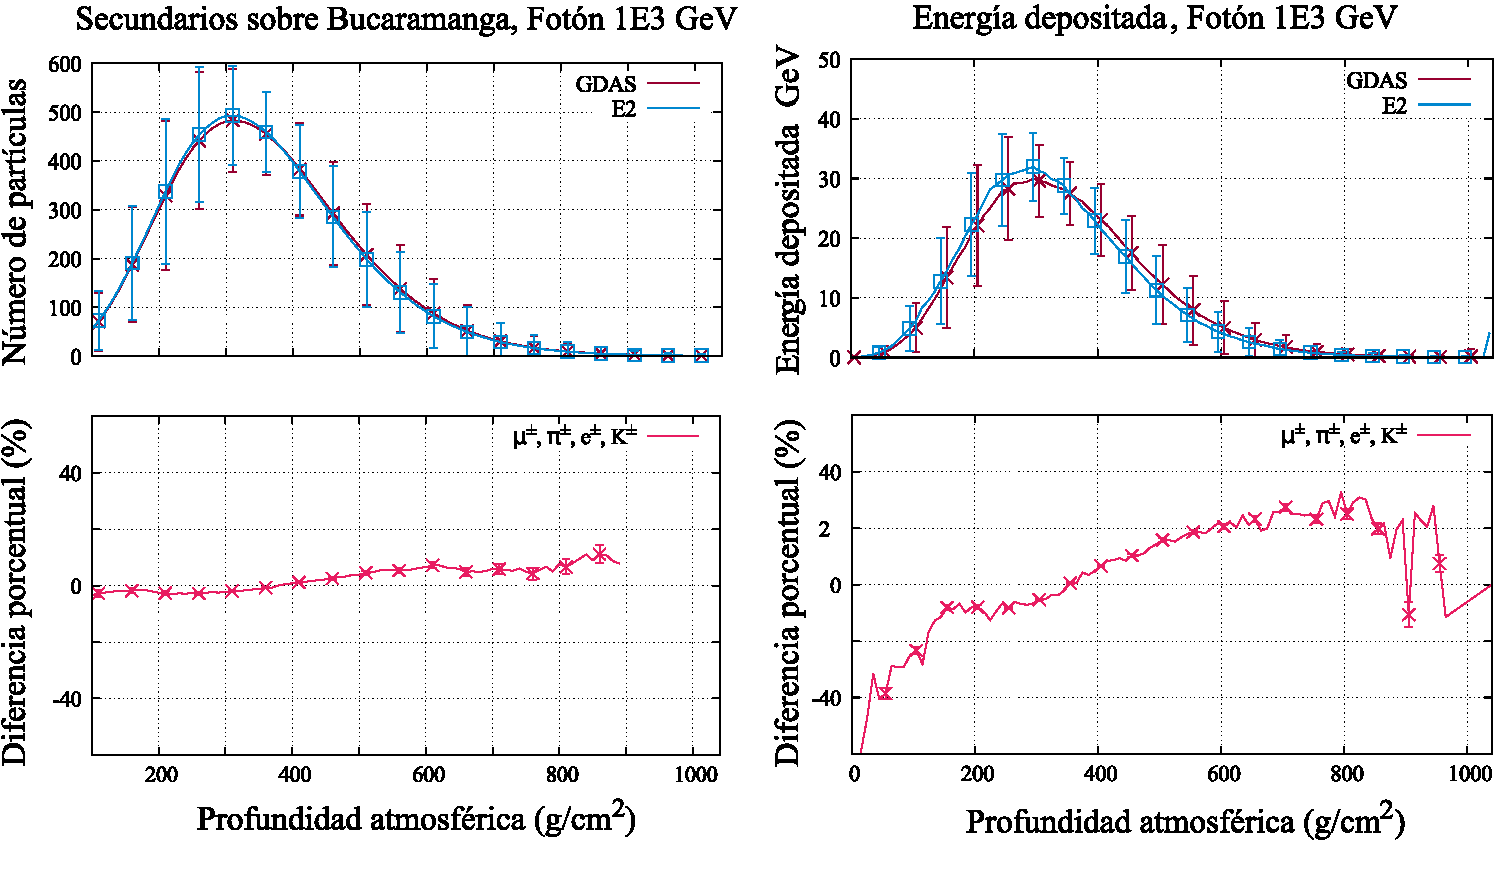
\includegraphics[width=0.8\textwidth]{Figs/foton_1E3.pdf}
\caption[Distribución longitudinal de un fotón de $1\cdot 10^{3}$ GeV.]{Distribución longitudinal de un foton de $1\cdot 10^{3} GeV$ que fue simulado 5000 veces, usando la atmósfera predeterminada (línea azul), y usando la atmósfera construida para el mes de abril (línea roja).}
\label{fig:fig30}
\end{figure}

\begin{figure}[htb!]
\centering
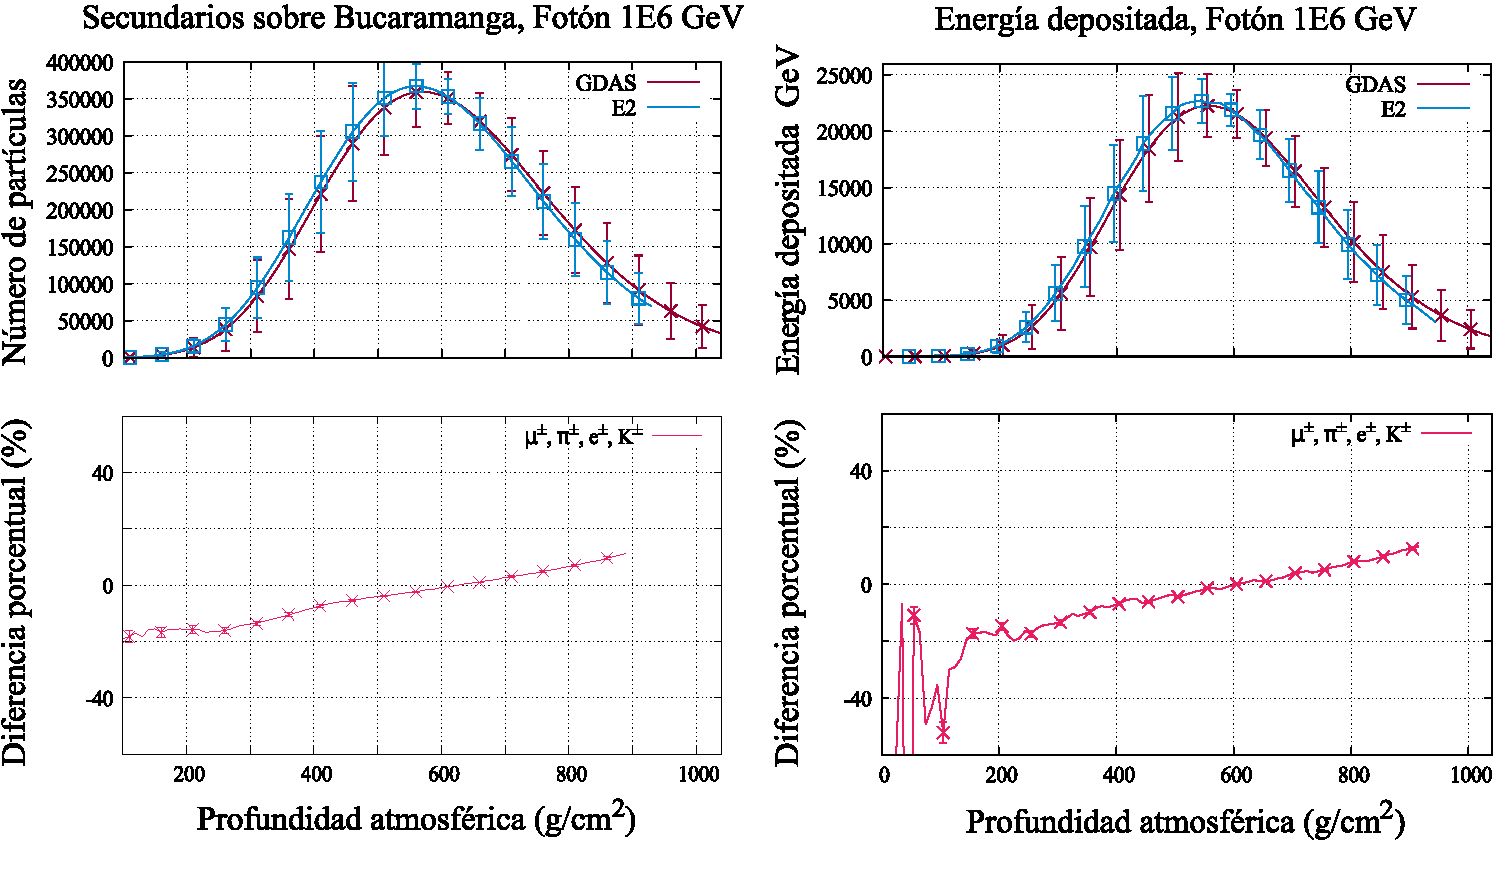
\includegraphics[width=0.8\textwidth]{Figs/foton_1E6.pdf}
\caption[Distribución longitudinal de un fotón de $1\cdot 10^{6}$ GeV.]{Distribución longitudinal de un fotón de $1\cdot 10^{6} GeV$ que fue simulado 1000 veces, usando la atmósfera predeterminada (línea azul), y usando la atmósfera construida para el mes de abril (línea roja). }
\label{fig:fig31}
\end{figure}

\begin{figure}[htb!]
\centering
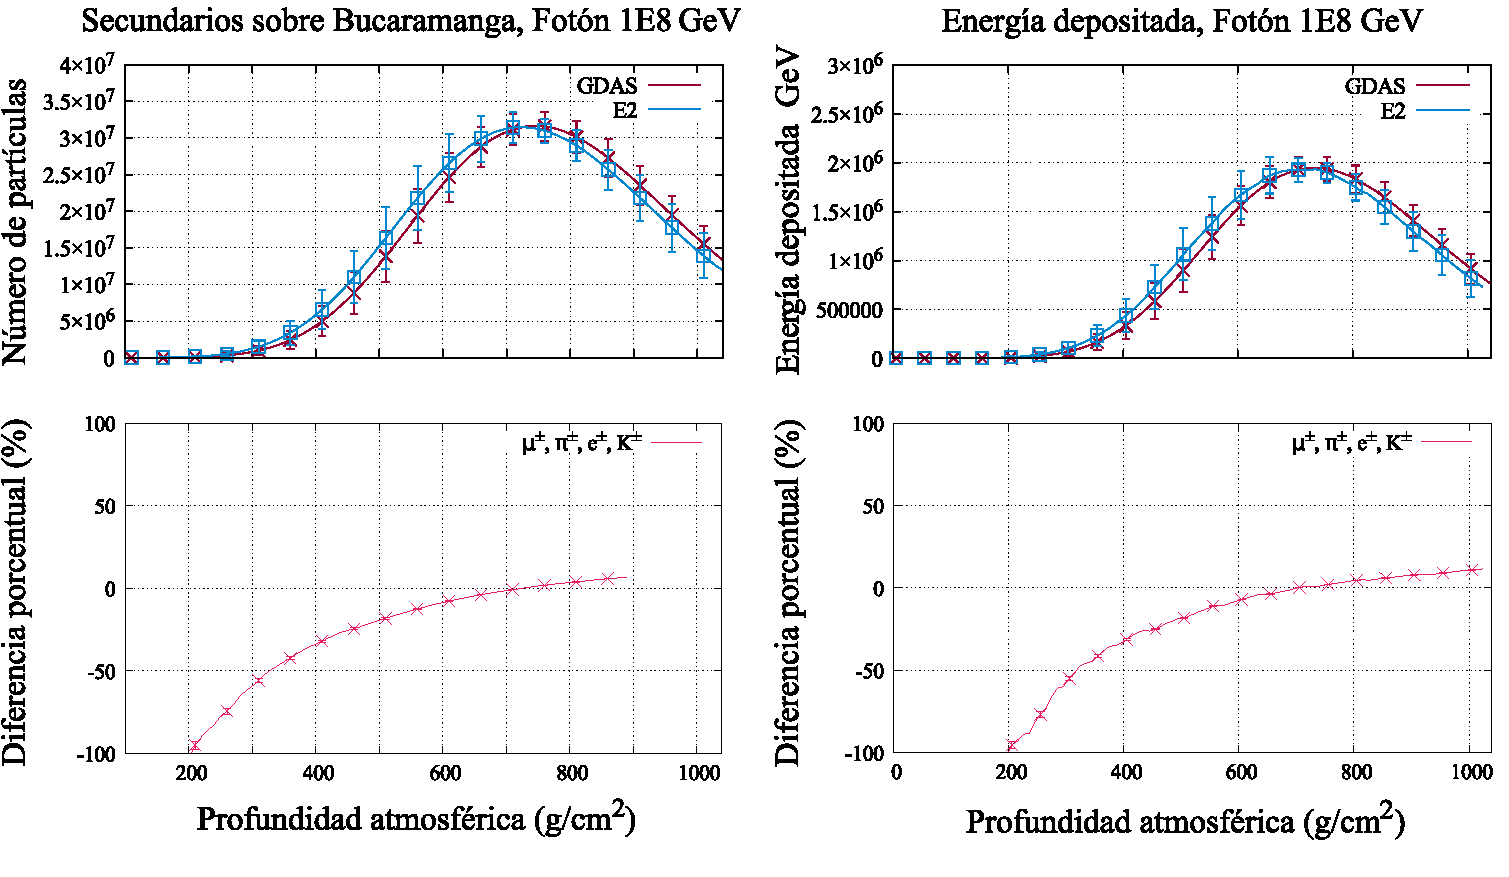
\includegraphics[width=0.8\textwidth]{Figs/foton_1E8.pdf}
\caption[Distribución longitudinal de un fotón de $1\cdot 10^{8}$ GeV.]{Distribución longitudinal de un fotón de $1\cdot 10^{8} GeV$ que fue simulado 10 veces, usando la atmósfera predeterminada (línea azul), y usando la atmósfera construida para el mes de abril (línea roja). }
\label{fig:fig32}
\end{figure}





